\documentclass[conference]{IEEEtran}
\IEEEoverridecommandlockouts
% The preceding line is only needed to identify funding in the first footnote. If that is unneeded, please comment it out.
\usepackage{cite}
\usepackage{amsmath,amssymb,amsfonts}
\usepackage{algorithmic}
\usepackage{graphicx}
\usepackage{textcomp}
\usepackage{xcolor}
\usepackage{algorithm}
\def\BibTeX{{\rm B\kern-.05em{\sc i\kern-.025em b}\kern-.08em
    T\kern-.1667em\lower.7ex\hbox{E}\kern-.125emX}}
\begin{document}

\title {An Analysis of Government ID’s Implemented using NFTs \\[1ex] \large https://github.com/abdullahsalous/An-analysis-of-Government-ID-s-implemented-using-NFTs \\[1ex] \large https://www.youtube.com/}

\author{\IEEEauthorblockN{Abdullah Salous}
\IEEEauthorblockA{\textit{Computer Science} \\
\textit{University of Oklahoma}\\
Norman, United States \\
abdullah.r.salous-1@ou.edu}
}

\maketitle

\begin{abstract}
In the United States, traditional government-issued IDs such as driver's licenses, Social Security numbers, and passports are increasingly vulnerable to fraud, forgery, and data misuse. As a potential alternative, this paper explores the feasibility of a blockchain-based digital identification system using non-fungible tokens (NFTs). While the concept of on-chain identity is still emerging, several real-world implementations such as Proof of Humanity, Gitcoin Passport, and Polygon ID offer foundational insights. This study empirically analyzes these existing Web3 identity projects to identify their strengths, limitations, and technical design patterns. Additionally, the paper proposes a prototype schema for NFT-based identity credentials. The proposed approach will be compared against current U.S. ID systems, focusing on security, scalability, data minimization, and legal implications. The goal is to determine whether identity NFTs can practically enhance or complement national identity infrastructure in an effective way.
\end{abstract}

\section{Introduction}
In the age of technology, identity theft is an increasing and pertinent issue to many Americans. According to the Bureau of Justice Statistics, approximately 23.9 million U.S. residents aged 16 or older (9\% of the population) experienced identity theft in 2021, while nearly 1 in 5 adults reported having been victims at some point in their lives \cite{Bureau of Justice Statistics}. As illustrated in Figure \ref{fig:ID Theft}, data from the Federal Trade Commission shows a steady rise in reports of fraud, identity theft, and related issues over the past five years, with a significant spike in 2021. On average, identity theft alone accounts for approximately 300,000 reports each year. These incidents often involve the misuse of personal information such as Social Security numbers, driver's licenses, and bank details, leading to financial loss, legal complications, and long-term reputational damage. 

\begin{figure}[h!]
    \centering
    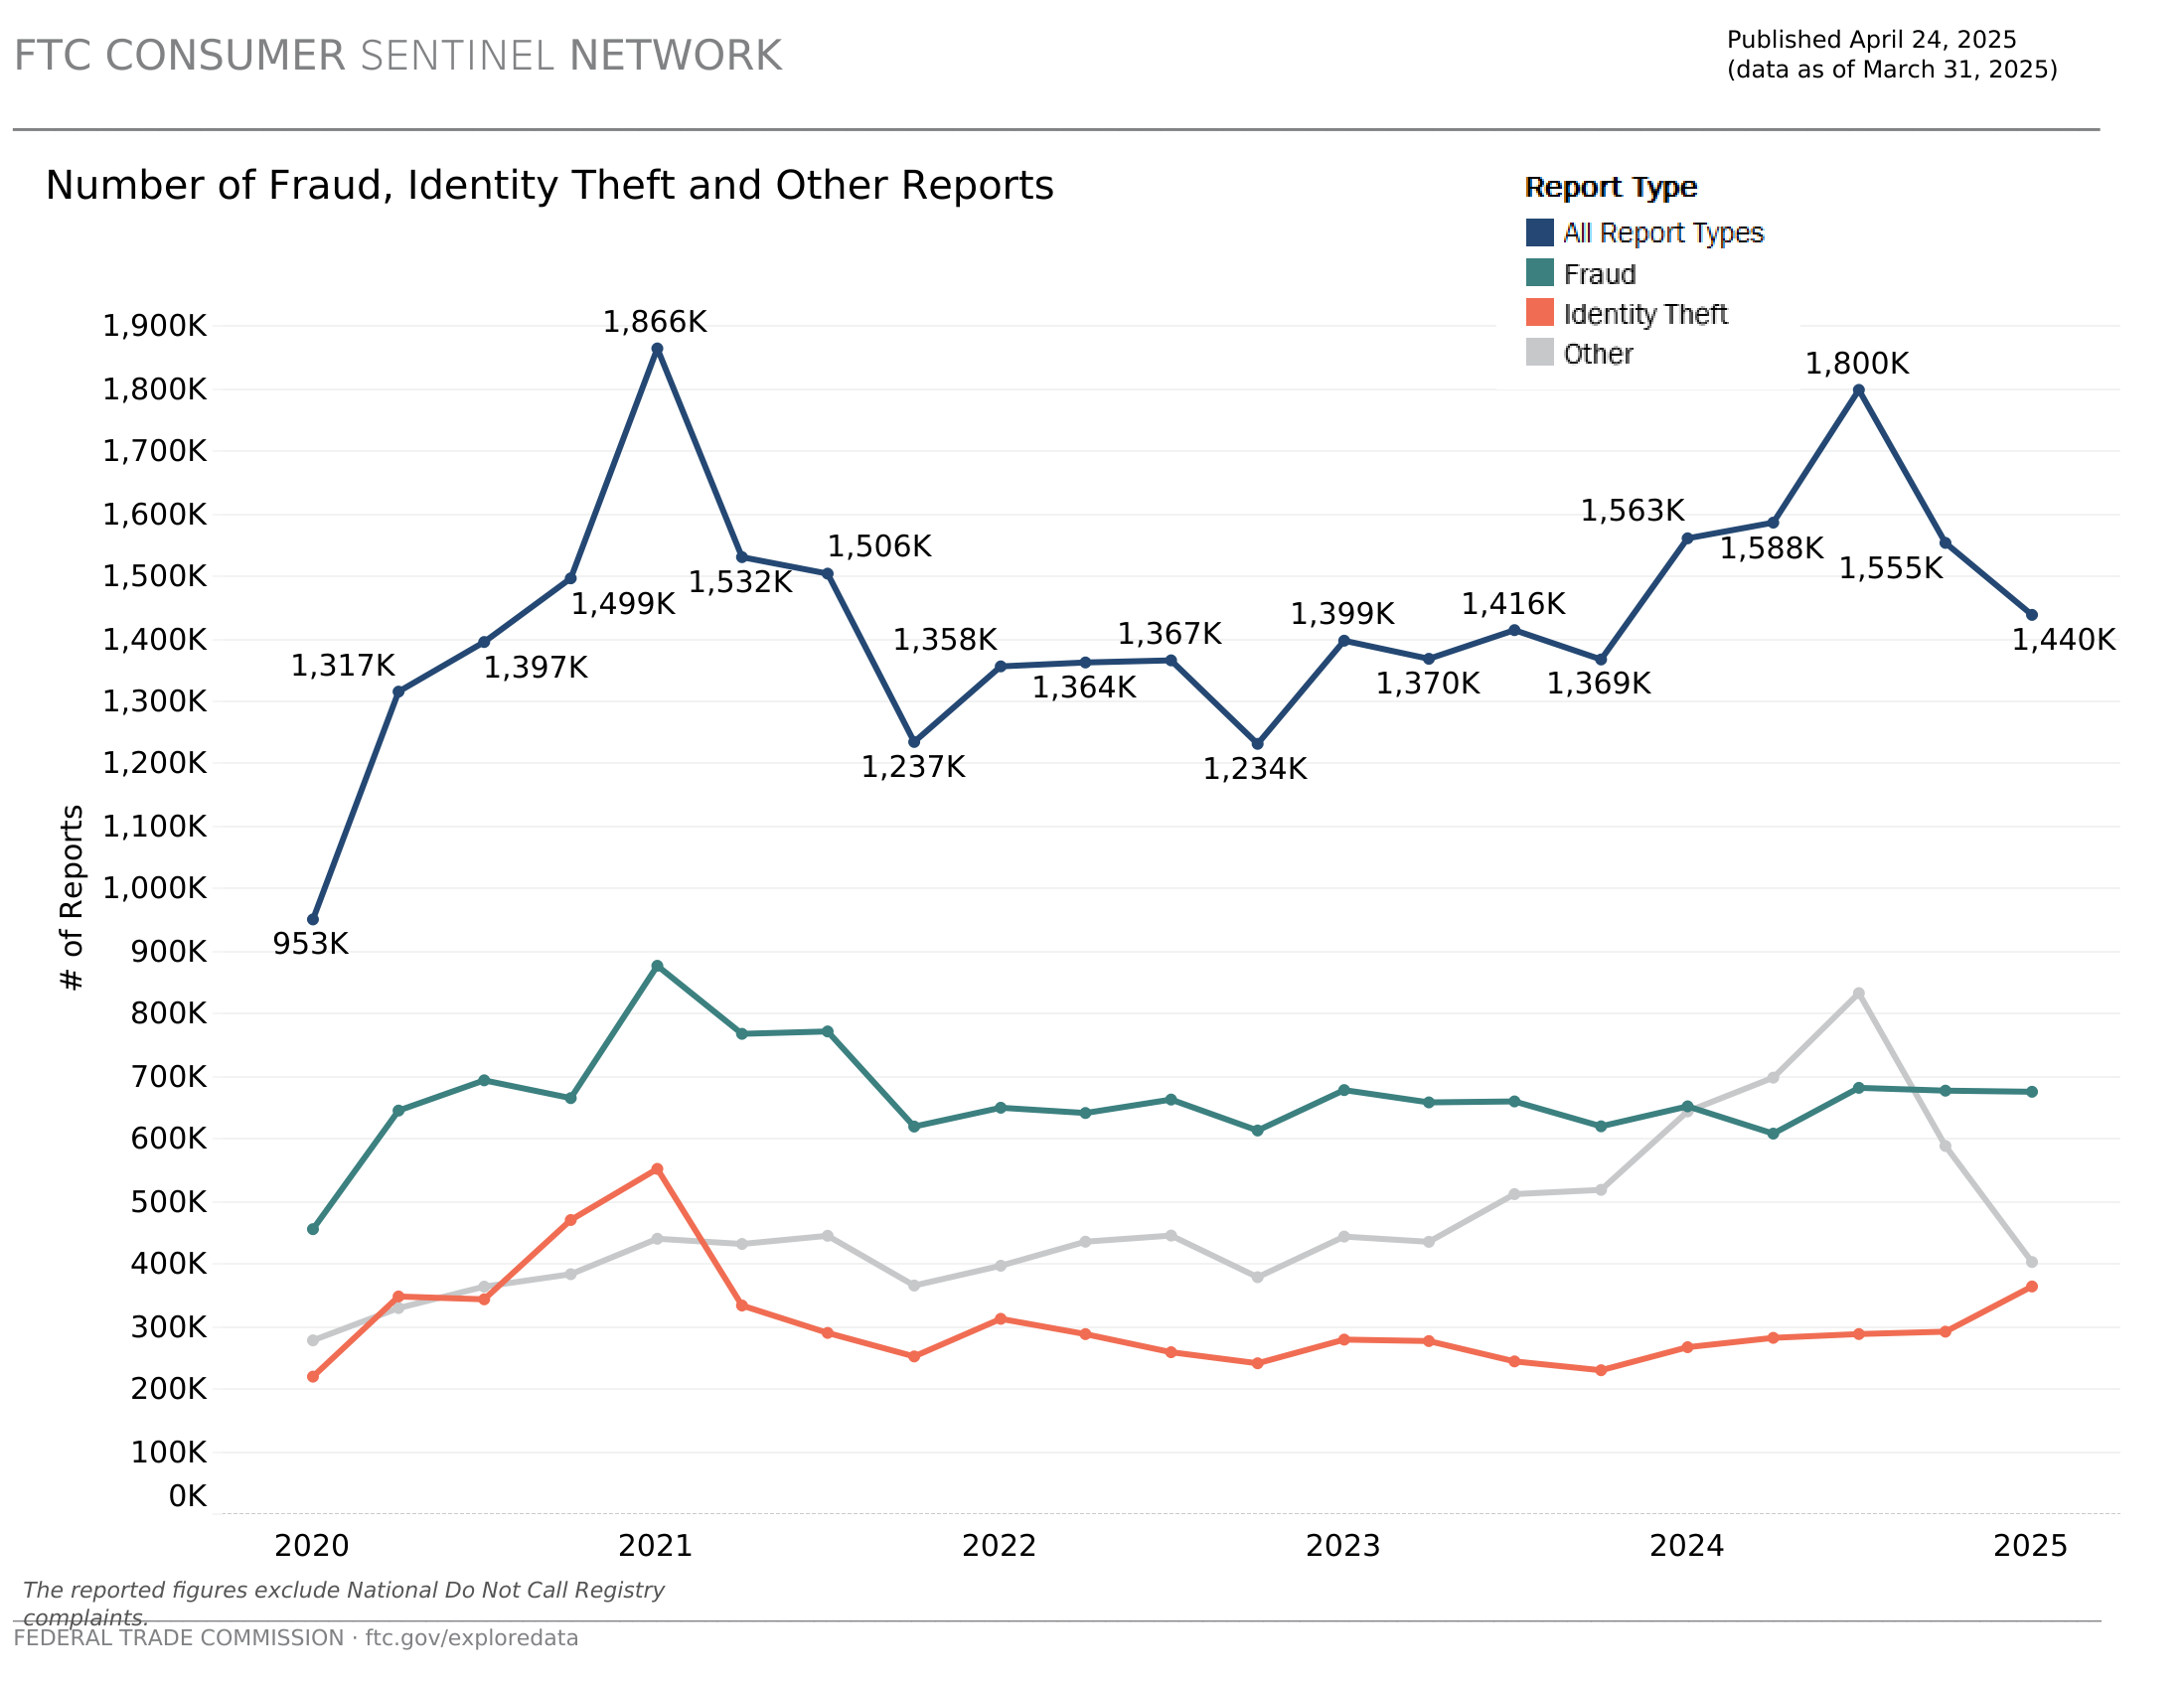
\includegraphics[width=0.9\linewidth]{Trends Over Time.png}
    \caption{Fraud, Identity Theft, and Other Reports}
    \label{fig:ID Theft}
\end{figure}

Despite the increasing sophistication of cybersecurity tools, traditional government-issued forms of identification remain vulnerable to theft, forgery, and data breaches. One significant concern is the widespread use of fake IDs, which are commonly used not only by underage individuals for age-restricted purchases, but also by criminals for more serious offenses such as identity fraud, illegal immigration, and financial scams. According to "IDScan.net", a study conducted found that 12.5\% of high school students admitted to possess a fake ID, and 32.2\% of college students under 21 admitted to possess it as well \cite{fake ID's}. As of 2024, CBS News reported that approximately 40,000 migrants from South and Central America entered the U.S. without authorization, with many resorting to purchasing counterfeit identification documents as a means of securing work to support their families \cite{cbs-news}. This shows the ease with which physical documents like driver's licenses or passports can be counterfeited or altered, thus highlights the limitations of document-based verification. Additionally, centralized identity repositories have proven to be high-value targets for cyberattacks. For instance, the 2015 breach of the U.S. Office of Personnel Management (OPM) compromised the personal data of over 21.5 million people \cite{opm}. These vulnerabilities expose structural weaknesses in existing systems and underscore the urgent need for more tamper-resistant, secure, and verifiable methods of identity management.

Blockchain technology, particularly through the use of non-fungible tokens (NFTs) presents a compelling alternative. These systems offer the promise of tamper-proof, self-sovereign digital identity that can be cryptographically verified and selectively disclosed by users. Several projects have begun experimenting with this concept, including Proof of Humanity, Gitcoin Passport, and Polygon ID, each offering a different take on how identity can be established and managed on-chain.

Despite these innovations, the integration of blockchain-based identity into national systems like that of the U.S. remains largely unexplored. This paper investigates whether NFT-based identity systems built on platforms like Ethereum could provide a more secure, privacy-preserving, and user-controlled framework for digital identification. By comparing blockchain-based identity models to current U.S. government systems, and by analyzing real-world blockchain data, this study aims to evaluate the feasibility of adopting such technology at scale.


\section{Background \& Related Work}
The internet is rapidly evolving with the emergence of Web3, a new phase defined by decentralization, user ownership, and cryptographic security. Unlike the current Web2 landscape, where user data is controlled by centralized platforms, Web3 empowers individuals to manage their own identities and digital assets without relying on third parties \cite{what-is-web3}. This shift introduces new possibilities for privacy-preserving and tamper-resistant identity systems. Several projects, such as Proof of Humanity, Gitcoin Passport, and Polygon ID, are already exploring how decentralized technologies can reshape how we approach identity authentication.

\subsection{Proof of Humanity}
Proof of Humanity (PoH) is a decentralized identity verification system designed to ensure that participants in a digital ecosystem are real, human individuals rather than bots \cite{what-is-poh}. As artificial intelligence grows increasingly capable of mimicking human behavior and speech, the need for reliable human verification has become more urgent. Proof of Humanity addresses this challenge by combining social verification with a reputation-based system on the Ethereum blockchain. There are many different implementations of Proof of Humanity. In this paper, we will explore a few of these implementations. 

The first implementation to examine is Proof of Humanity by Kleros. PoH by Kleros requires users to first connect an online wallet. The wallet address provided by the user is publicly linked to their identity. Then, the registration process begins. Registration requires a user to submit a name, photo, and video holding their wallet address. They are then vouched for by an existing verified member. This crowd-sourced, tamper-resistant approach can reduce the risk of Sybil attacks and fake accounts while giving users greater control over their online interactions. By removing the need for centralized authorities, Proof of Humanity by Kleros seeks to offer a trustable and scalable framework for authenticating digital identity in Web3.

\begin{figure}[h!]
    \centering
    
\includegraphics[width=0.9\linewidth]{poh-kleros.png}
    \caption{Proof of Humanity Registration}
    \label{fig:poh-kleros}
\end{figure}

Another implementation of Proof of Humanity is 


\section{Comparative Analysis}
Criteria for evaluation: tamper resistance, privacy, scalability, data minimization, revocability, and legal compatibility
Evaluation of current U.S. ID system based on those criteria
Evaluation of blockchain-based identity systems using real-world data and documentation

\section{Prototype Design}

\section{Conclusion}


\begin{thebibliography}{00}
\bibitem{Bureau of Justice Statistics}“Victims of identity theft, 2021,” Bureau of Justice Statistics, https://bjs.ojp.gov/press-release/victims-identity-theft-2021. 

\bibitem{fake ID's}D. Papich, “How common are fake ids?,” IDScan.net,
https://idscan.net/blog/how-common-are-fake-ids/?srsltid=AfmBOoqOPSxNFDdifCClManqCJyKoqzAF2s6jpc2qWSBfe4UzCP-ylch

\bibitem{cbs-news}K. Weis, “Criminals selling fake identity documents to migrants in Colorado desperate to find work, CBS News Colorado Investigation finds,” CBS News, https://www.cbsnews.com/colorado/news/criminals-selling-fake-identity-documents-migrants-colorado-desperate-find-work-cbs-news-colorado-investigation-finds/. 

\bibitem{opm}J. Bracy, IAPP, https://iapp.org/news/a/21-5-million-breached-in-second-opm-hack. 

\bibitem{what-is-web3}P. Shoemaker, “What is web3? web 3.0 explained,” Identity, https://www.identity.com/web3/.

\bibitem{what-is-poh}P. Shoemaker, “Why proof of humanity is more important than ever,” Identity, https://www.identity.com/why-proof-of-humanity-is-more-important-than-ever/.

\end{thebibliography}

\end{document}
